\chapter{Convolutional Neural Networks}
\label{chapter:intro}
\section{CNN(Convolutional Neural Networks)介紹}
卷積神經網路(Convolutional Neural Network)為深度學習的分類模型,是一種前饋神經網路,對於大型圖像處理有出色表現,架構為一輸入層、數個隱藏層與一輸出層所組成,其中隱藏層包含有卷積層、池化層與全連接層。它與多層感知器不同點是並非所有神經元會全部連結。訓練過程是從訓練集中以梯度下降法來確定權重與偏差。
\begin{figure}[H]
	\centerline{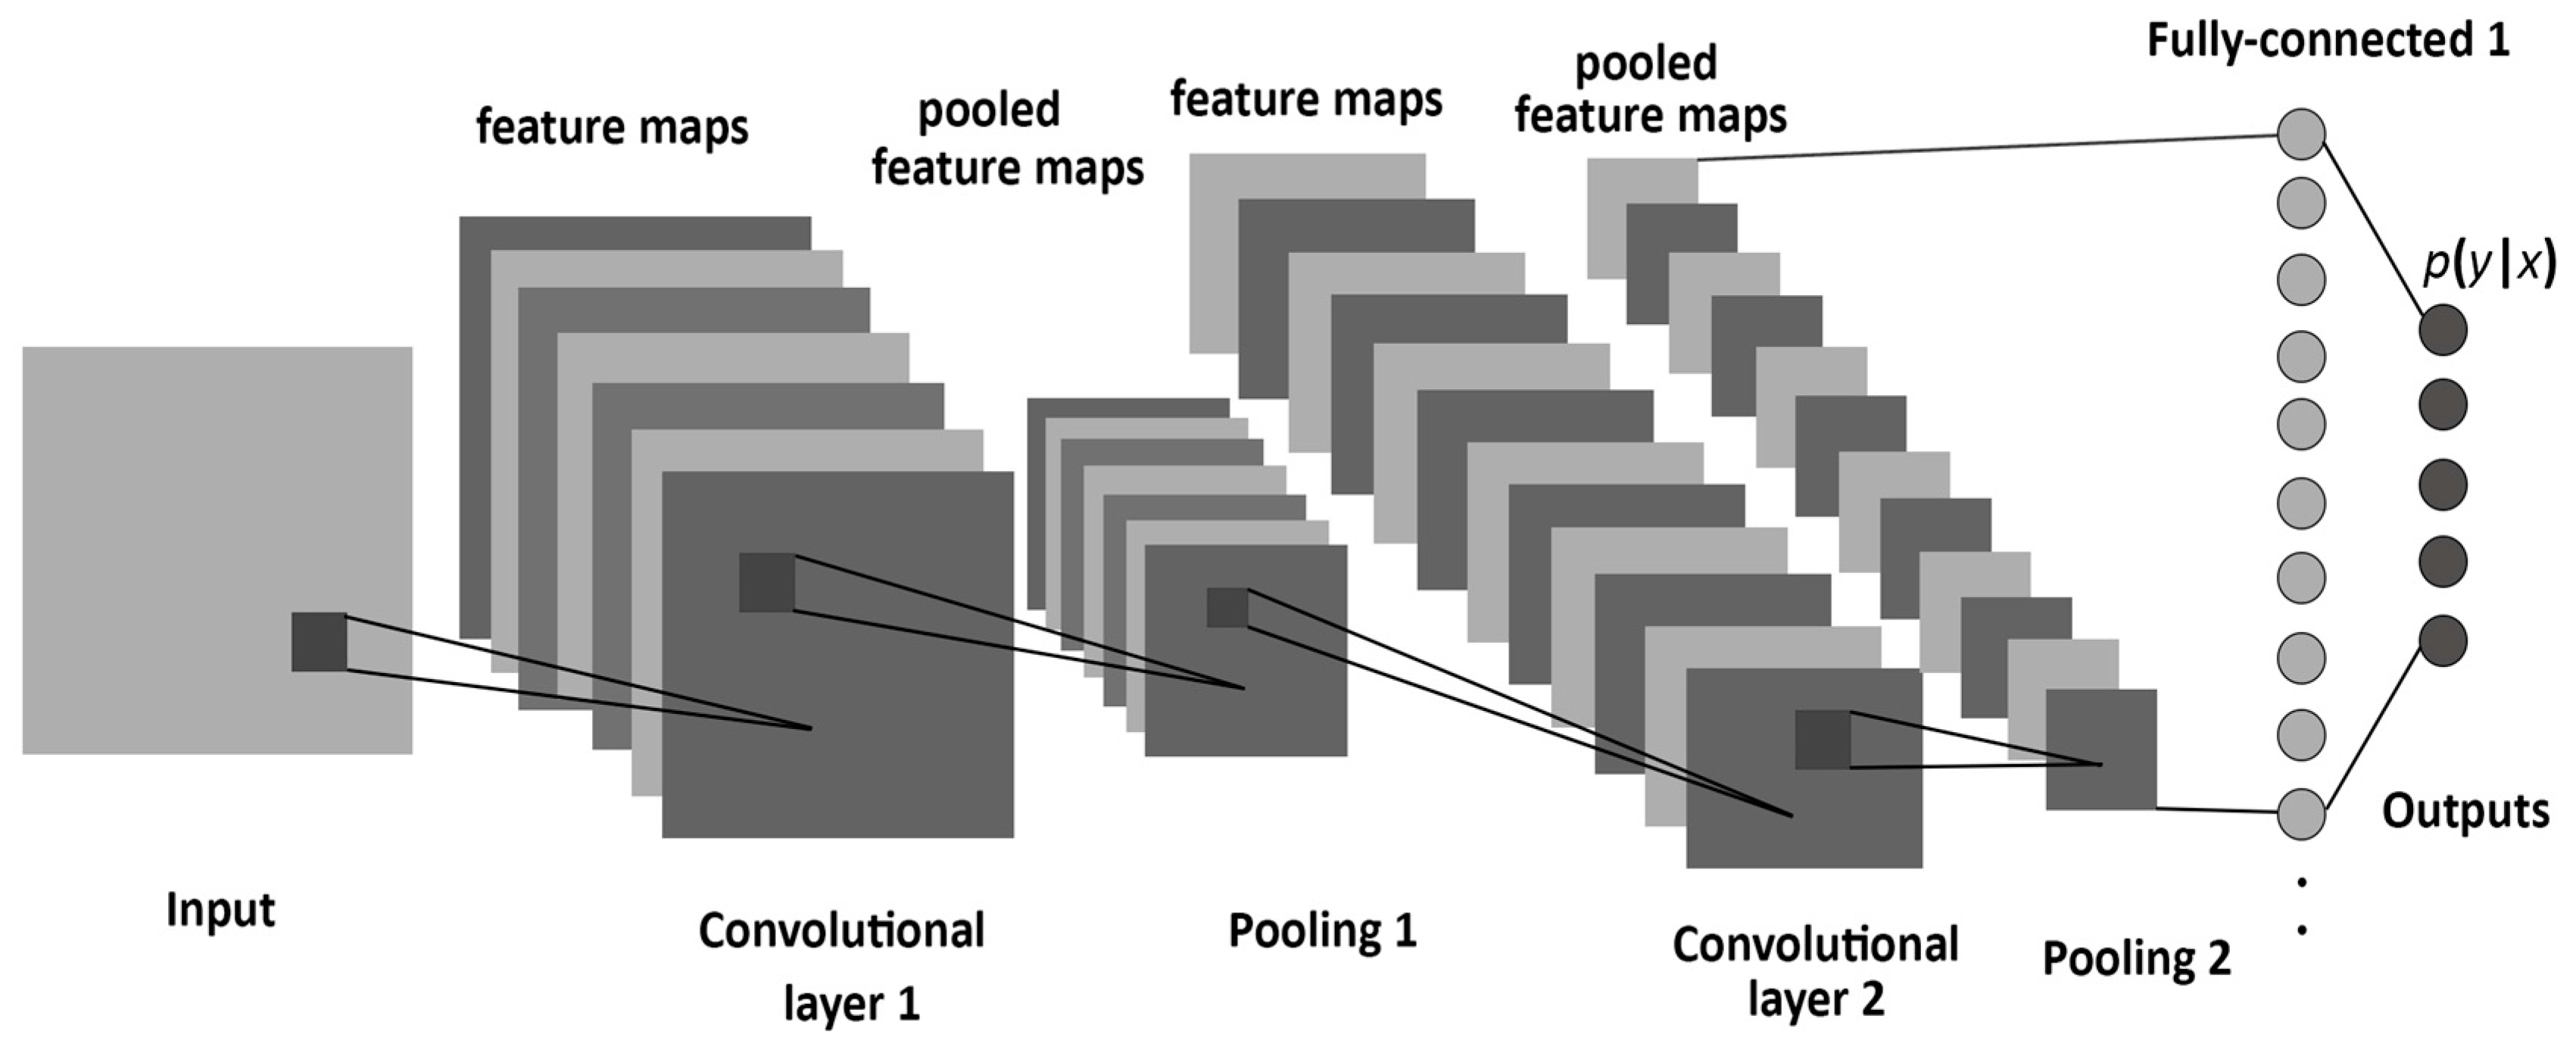
\includegraphics[height=7cm]{pic/CNNAR.png}}
	\caption{CNN架構圖}
	※引用:Saleh Albelwi and Ausif Mahmood(2017)。A Framework for Designing the Architectures of Deep Convolutional Neural Networks

	\label{fig:CNNArchiteture}
\end{figure}


\label{sec:background}
\section{CNN(Convolutional Neural Networks)基本結構}
\subsection{輸入層(Input Layer)}
用於數據的輸入。
\subsection{卷積層(Convolution Layer)}

尋找特徵,CNN是根據影像的特徵來判別分類,不必由整個影像來判別。因為共用相同的特徵參數,如果對上不同影像,只要有相同的特徵出現,就算在不同的區域依然可以找到。利用遮罩(Mask)在原始影像上移動,濾波器的值對遮罩內的值作內積計算,這過程稱為卷積(Convolution)。

%\begin{itemize}
%	\item 
%
%\end{itemize}


圖\ref{fig:Convolution}與圖\ref{fig:ConvolutionFinally},第一格的計算如式\ref{eqn:ConvolutionCaculate}結果為1。一次往右一格以此類推進行計算,到邊界時往下一列從新的一行開始計算,最後得出卷積(Convolution)結果。

\begin{equation}
	\label{eqn:ConvolutionCaculate}
	2\times(-1)+2\times0+0\times0+0\times0+1\times0+1\times0+0\times1+1\times0+2\times1+1\times1=1
\end{equation}


\begin{figure}[H]
	\centerline{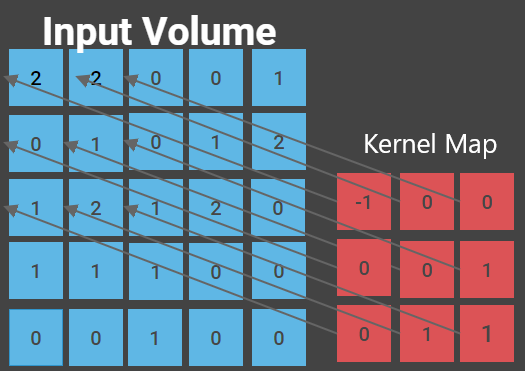
\includegraphics[height=5cm]{pic/CNN1.png}}
	\caption{卷積(Convolution)示意圖}
	\label{fig:Convolution}

	\centerline{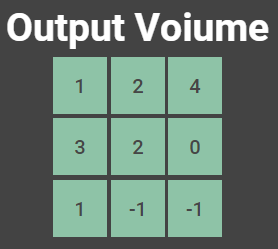
\includegraphics[height=5cm]{pic/CNN2.PNG}}
	\caption{卷積(Convolution)結果示意圖}
	\label{fig:ConvolutionFinally}
\end{figure}


\newpage
具有特徵的濾波器內的權重其數值取得,一開始設置初始權重,因為一開始特徵並不是最好的特徵,因此模型預測與標籤所計算的誤差會非常高。但透過梯度下降法更新濾波器的權重,隨著訓練多次迭代,它會自動趨近於它認為最好的特徵,這特點稱為自動提取特徵。


卷積前後影像大小改變:

是否進填充將影響影像大小的改變,上述例子是採用VALID padding,如圖\ref{fig:Convolution},不在原有的影象基礎上做任何填充,但這樣會有個缺點,在卷積多次後,可能使邊緣的畫素和卷積核做卷積的次數小於影象中間的畫素點,從而導致對其資訊的特徵的提取不足。


所以另一個方法SAME padding,使得做卷積運算後,原始影象的大小會保持原樣。

填充的大小計算公式:
\begin{equation}
	\label{eqn:Padding}
	P=(F-1)/2
\end{equation}

\begin{itemize}
	\item
	      P為填充

	\item
	      F為卷積核的寬 ( 高 ) 度
\end{itemize}


\begin{figure}[H]
	\centerline{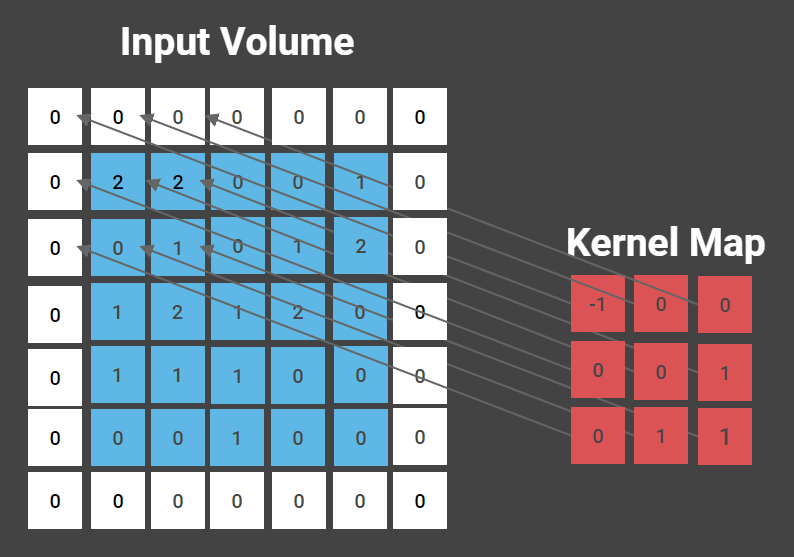
\includegraphics[height=5cm]{pic/samepadding.PNG}}
	\caption{卷積(Convolution)有填充示意圖}
	\label{fig:SamePadding}
\end{figure}
\begin{figure}[H]
	\centerline{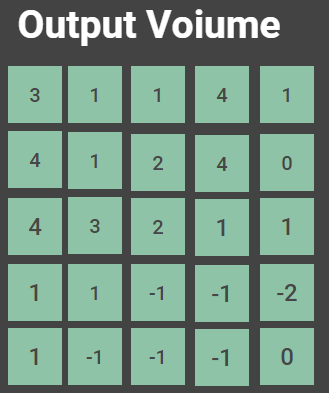
\includegraphics[height=5cm]{pic/samepaddingout.PNG}}
	\caption{卷積(Convolution)有填充結果示意圖}
	\label{fig:SamePaddingOutcome}
\end{figure}


卷積前後影像大小計算:
\begin{equation}
	\label{eqn:ImageShapeAfterConvolution}
	Woutput=(Winput-F+2P)/S+1
\end{equation}

\begin{itemize}
	\item
	      Woutput為特徵圖的寬 ( 高 ) 度
	\item
	      Winput為前圖像寬 ( 高 ) 度
	\item
	      F為卷積核的寬 ( 高 ) 度
	\item
	      P為填充,使用填充:原始影像周圍補上零
	\item
	      S為步長(每次移動遮罩的距離)
\end{itemize}

圖\ref{fig:Convolution}是 \(5 \times5\)的影像,經過\(3 \times 3\)濾波器每次一步,不進行填充卷積後影像為圖\ref{fig:ConvolutionFinally},計算大小(5-3+2*0)/1+1=3,卷積後影像大小為 \(3 \times 3\) 


圖\ref{fig:SamePadding}是\(5 \times 5\)的影像經過\(3 \times 3\)濾波器每次一步,進行填充,卷積後影像為圖\ref{fig:SamePaddingOutcome},計算大小(5-3+2*1)/1+1=5,卷積後影像大小為 \(5 \times 5\)




\subsection{池化層(pooling Layer)}
對影像進行欠取樣(Undersampling)使影像大小在不改變特徵時減少像素,達到減少運算時的數據量。
上述方法稱為:池化,池化是先在圖片上選取不同窗口(window),並在這個窗口範圍中依據不同方法選擇一個特徵值。

如果是使用\(2 \times 2\)的窗口,原圖經過池化以後,其所包含的像素數量會降為原本的四分之一,如圖\ref{fig:PoolingLayer}中 \(6 \times6\) 的圖檔經過\(2 \times 2\)的窗口進行池化,變成\(3 \times 3\)的特徵圖
但因為池化後的圖片包含了原圖中各個範圍的特徵值,保留了每個範圍內各個特徵的相符程度。池化後的資訊更專注於圖片中是否存在相符的特徵,而非圖片中哪裡存在這些特徵。這能幫助 CNN 判斷圖片中是否包含某項特徵,而不必分心於特徵的位置。

\begin{itemize}
	\item
	      最大池化(Max Pooling):
取所有元素的最大值。如圖\ref{fig:PoolingLayer}第一個窗口數字為[0.8,0.7,1,0.5] 局部最大池化選取所有元素的最大值,此窗口最大值為1,選擇1為特徵值。
	\item

	      平均池化(Average Pooling):取所有元素的平均值。如圖\ref{fig:PoolingLayer}第一個窗口數字為[0.8,0.7,1,0.5] 局部平均池化選取所有元素的平均值,所以(0.8+0.7+1+0.5)/4=0.75,所以選擇0.75為特徵值。
\end{itemize}




\begin{figure}[H]
	\centerline{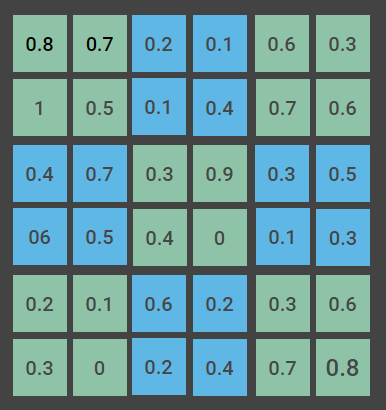
\includegraphics[height=7cm]{pic/pooling 1.PNG}}

	\caption{Pooling Layer示意圖}
	\label{fig:PoolingLayer}
\end{figure}
\begin{figure}[H]
	\centerline{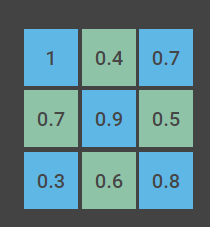
\includegraphics[height=5cm]{pic/poolinig 2.PNG}}
	\caption{Max Pooling示意圖}
	\label{fig:MaxPooling}
\end{figure}
\begin{figure}[H]
	\centerline{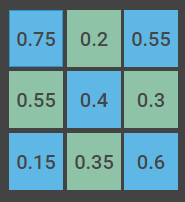
\includegraphics[height=5cm]{pic/pooling 3.PNG}}
	\caption{Average Pooling示意圖}
	\label{fig:AveragePooling}
\end{figure}


\subsection{全連接層(Fully Connected Layer)}
將所有特徵圖變為一維度,並組合在一起來進行輸出分類,簡單的來說就是一個分類器,把我們經過數個卷積、池化後的結果進行分類。
把我們經過數個卷積、池化後的結果進行分類。通 常 在 全 連 接 層 與 輸 出 層 間 會 使 用 Softmax(歸一化指數函式)函數來輸出機率,使所有類別的機率和為1。
它能將一個含任意實數的K維向量「壓縮」到另一個K維實向量 中,使得每一個元素的範圍都在(0,1)之間,並且所有元素的和為1。
Softmax公式\ref{eqn:Softmax}
\begin{equation}
	\label{eqn:Softmax}
	\sigma(z)_j=\frac{e^{z_j}}{\sum_{k=1}^{K}e^{zk}} \ \ \ \ \ \ \ \ \ for\ 1,....,K
\end{equation}


\section{CNN(Convolutional Neural Networks)訓練過程與參數設定}
\subsection{演算法參數}
model.add=(Convolution2D(output size,Kernal Size,padding方法,input shape =(img channels,img rows,img cols))
model.add(激活函數)
\begin{enumerate}
	\item
	      輸入圖片:img channels:圖片類別,img rows,img cols:圖片的寬高
	\item
	      設定卷積核大小Kernal Size(6,6)
	\item
	      output size:卷積後的深度
	\item
	      padding方法:有VALID padding和SAME padding
	\item
	      激活函數使用ReLU函數,式\ref{eqn:ReLU}
	      \begin{equation}
		      \label{eqn:ReLU}
		      Relu(x)=
		      \left\{\begin{matrix}
			      x \ \ \ \ \ \ if\ x>0
			      \\
			      0 \ \ \ \ \ \ if\ x<0
		      \end{matrix}\right.
	      \end{equation}
\end{enumerate}
CNN演算法如圖\ref{fig:Keras}所示
\begin{figure}[H]
	\centerline{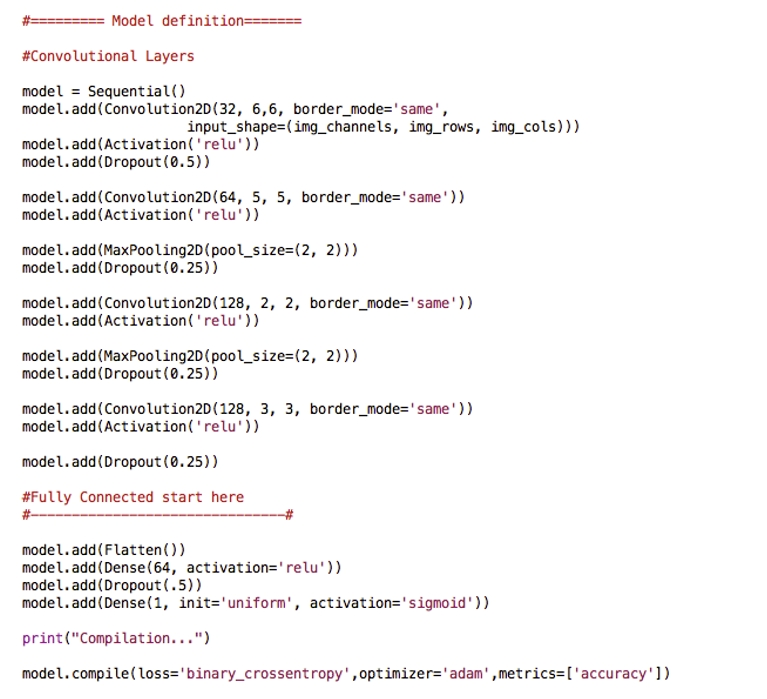
\includegraphics[height=15cm]{pic/Keras.jpg}}
	\caption{CNN演算法圖}
	\label{fig:Keras}
\end{figure}

\subsection{CNN(Convolutional Neural Networks)訓練過程}
\begin{enumerate}
	\item
	      初始化網絡權重。
	\item
	      輸入數據經過卷積層、池化層、全連接層的向前傳播得到輸出值。
	\item
	      求出網絡的輸出值與目標值之間的誤差,判斷是否達到設定的訓練目標。
	\item
	      並將誤差傳回網絡中,反向求得全連接層,池化層,卷積層的誤差。
	\item
	      根據求得誤差進行權重更新,用更新的權重進行回到第二步。
\end{enumerate}
\begin{figure}[H]
	\centerline{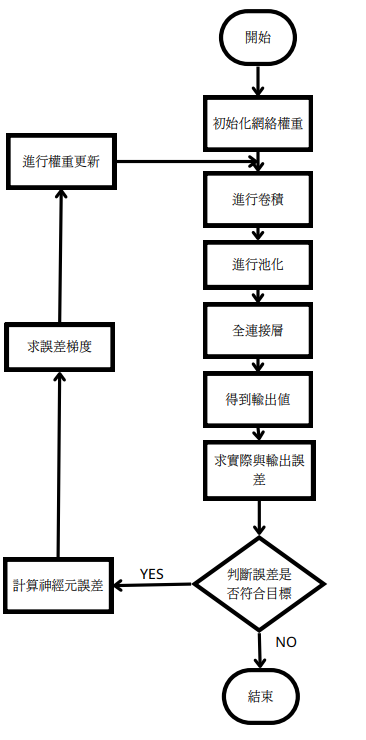
\includegraphics[height=15cm]{pic/CNNp.PNG}}
	\caption{CNN訓練流程圖}
	\label{fig:CNNTrainningFlowChart}
\end{figure}
\section{CNN(Convolutional Neural Networks) 結語}
卷積神經網路,因為可以進行局部權重共享的特殊性質,在圖形辨識方面有著獨特的優勢,權重共享降低了網路的複雜性,特別是在處理多維輸入的向量圖像,只要有鄰近資料相關性,三維或多維度的資料也都可以使用。
